% fitResults LaTeX beamer setup
%
% Copyright (C) 2014 Alex J. Grede
% GPL v3, See LICENSE.txt for details
% This function is part of <NAME> (https://github.com/agrede/<GITHUB>)
\documentclass{beamer}
\usepackage[utf8]{inputenc}
\usepackage[T1]{fontenc}
\usepackage[]{graphicx}
\usepackage{helvet}
\usepackage{amssymb}
\usepackage{amsmath}
\usepackage{textcomp}
\usepackage{latexsym}
\usepackage{mathrsfs}
\usepackage{csquotes}
\usepackage{tabularx}
\usepackage[use-xspace=true,range-units=single]{siunitx}
\usepackage[version=3]{mhchem}

\definecolor{'pca'}{HTML}{7788B1}
\definecolor{'pcb'}{HTML}{4A4E58}
\definecolor{'pcc'}{HTML}{001035}
\definecolor{'pcd'}{HTML}{D5E2FF}
\definecolor{'pce'}{HTML}{FFFFFF}

\definecolor{barblue}{RGB}{153,204,254}
\definecolor{groupblue}{RGB}{51,102,254}
\definecolor{linkred}{RGB}{165,0,33}

\useoutertheme{infolines}
\usecolortheme[RGB={119,136,177}]{structure}
\usetheme{Rochester}
\setbeamertemplate{items}[default]
\setbeamertemplate{blocks}[shadow=false]
\setbeamertemplate{navigation symbols}{}
\sisetup{
  table-number-alignment=center,
  tight-spacing=true
}

\renewcommand*{\familydefault}{\sfdefault}

\title[Diode Fits]{Diode Fits}
\author[Grede]{Alex J. Grede}
\institute[RIT]{Rochester Institute of Technology}
\date{\today}

\begin{document}

\begin{frame}
\titlepage
\end{frame}

\section{Model}
\label{sec:model}


\begin{frame}
  \title{Model and Residual}
  \begin{columns}[T]
    \begin{column}{0.45\textwidth}
      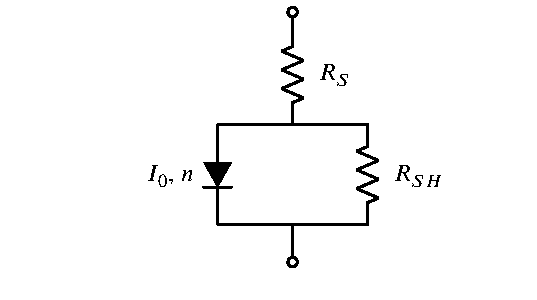
\includegraphics[width=\textwidth]{model}
    \end{column}
    \begin{column}{0.45\textwidth}
      \begin{equation}
        \label{eq:1}
        r_{k} = \left( \log\left( I_{k} \right) - \log \left( I\left( V_{k} \right) \right) \right)^2
      \end{equation}
    \end{column}
  \end{columns}
\end{frame}

\input{results}

\end{document}

%%% Local Variables:
%%% mode: latex
%%% TeX-master: t
%%% End:
